% Chapter Template

\chapter{Introduction} % Main chapter title

\label{Introduction}


\section{Problem}
Human pose estimation is a task based on a human's image or 3D points, and the model should locate the main joints in the human's body (head, neck, left and right arms, spin, etc.) as shown in the Figure  \ref{example}. Each joint is represented as a point in 2D or 3D space based on the task's objective.

\begin{figure}[htbp]
\centerline{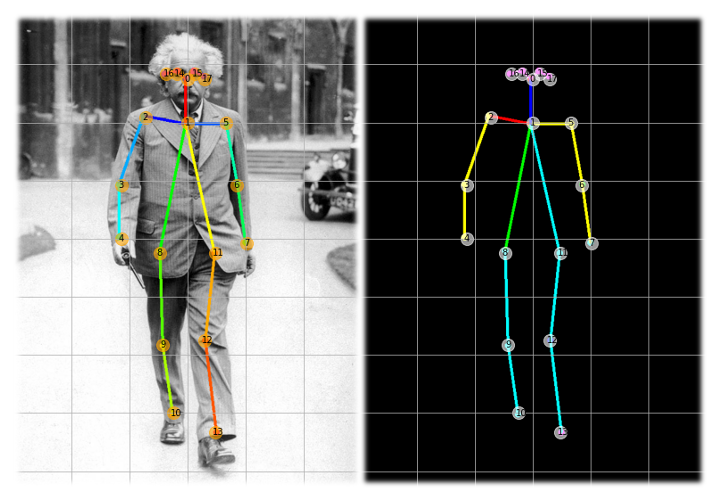
\includegraphics[scale=.5]{Figures/introduction-einstein.png}}
\caption{Example of human pose estimation key points \cite{rovai_realtime_2020}}
\label{example}
\end{figure}

A 3D point cloud is simply a set of points with three positional coordinates and represents points in 3D space. The points represent the shape of the object in 3D space. 3D point clouds are usually gathered by 3D scanners or dual-lens cameras.The output of scanners is point cloud where each point corresponds to some point on scanning surface with predefined precision. With the rapid growth of LIDAR and VR fields, the importance of accurate and fast 3D point cloud human pose estimation algorithms is clear.

\section{Challenges}
The obvious challenge of human pose estimation is the potential space of different human postures. The small change in the body part position changing the target pose. The task gets more complicated with different obstacles like clothes.
Using recent ML algorithms such as deep learning on 3D point cloud results in many challenges. Some of the common issues are:
\begin{itemize}
  \item The high dimensionality of the input space. Compared to pose estimation based on images, 3D point cloud has higher-dimensional space.
  \item Noisy inputs from 3D point cloud scanners. The sparsity and accuracy of the point cloud greatly influence the model's performance. The accuracy and granularity of points are significantly dependent on the scanning device. Compact LIDAR scanning devices the most popular and less accurate.
  \item Geometric-viewpoint relation. The human body has a strict geometric relation between body parts, which is invariant to the viewpoint. Most of the deep learning algorithms are not viewpoint agnostic resulting in additional challenges for human pose estimation.
  \item Lack of data. The amount of data for 3D point cloud human pose estimation is significantly less than regular image datasets. This fact is due to the high complexity of collecting 3D point cloud data, e.g., need special multicamera or LIDAR equipment, need diverse human positions, need different human constitutions.
\end{itemize}

\section{Motivation}
Human pose estimation is an important task that is used in different fields.
A lot of research work was done to solve the task of human pose estimation using point clouds. These works made significant progress in the regression task and showed good performance on public datasets. However, most methods use the end-to-end approach of learning, paying less attention to the inner structure of point cloud objects. The mutual relationship between an object's parts (in our case human body) plays a crucial role during the regression. 
The recent works \parencite{cheraghian_3dcapsule_2018,wu_3d_2020} which use capsule-based methods for point clouds, show that these types of models could consider object's part relationships. Moreover, auto-encoder capsule-based networks could learn objects' properties in unsupervised manner \parecite{wu_3d_2020}. These properties of capsule networks look promising for tasks where viewpoint invariance is a substantial challenge.
Moreover, some experiments \parencite{wang_capsule_2020,gritsevskiy_capsule_2018} stated that capsule networks need less data for convergence compared to non-capsule models. Besides, it is more noise agnostic than regular convolutional networks due to latent space inside the capsule network.

\section{Research Gap}
\begin{itemize}
  \item There is no capsule-based model for 3D human pose estimation task.
  \item There is no comparison of the influence of noisy data on capsule-based and non-capsule-based models for 3D space.
  \item There is no comparison of how well capsule-based works with limited dataset compared to regular models.
\end{itemize}

\section{Objective}
The work's objective is to propose a model based on a capsule network for a 3D point cloud human pose estimation. Evaluate the model on public benchmark dataset for human pose estimation. Compare results with state of the art approaches for the task as mentioned earlier. Evaluate the influence of the noise in training dataset on capsule-based and non-capsule-based networks. Measure the performance of the models with different sizes of training dataset.

\section{Paper structure}
Section \ref{Related work} covers the related work of human pose estimation based on both 2D images and 3D point clouds. This section described conventionally, and state of the art approaches for solving the issue. Reviews capsule networks for different 3D point cloud tasks like point classification, segmentation, and position estimation.

The rest of the paper is organized in the following manner:
\begin{itemize}
  \item Section \ref{Hypothesis} presents the project's hypothesis and problems;
    \item  section \ref{Dataset} describes the dataset which is used for training and evaluation along with evaluation metrics;
  \item  section \ref{Methodology} describes the approach for solving the project's objectives;
   \item  section \ref{Experiments} describes experiments on project's objections described in \ref{Methodology};
  \item  section \ref{Conclusions} sums up the paper's ideas and present brief conclusions and possible future work in this field.
\end{itemize}